%%%%%%%%%%%%%%%%%%%%%%%%%%%%%%%%%%%%%%%%%%%%%%%%%%%%%%%%%%%%%%%%%%%%%%%%%%%%%%
%
%%%%%%%%%%%%%%%%%%%%%%%%%%%%%%%%%%%%%%%%%%%%%%%%%%%%%%%%%%%%%%%%%%%%%%%%%%%%%%
% vim: set fenc=utf-8 ff=unix sw=2 tw=78 spell spl=fr :

\section {Analyse et phénomène linguistique}

Dans cette première partie nous allons succesivement présenter le phénomène linguistique, les motivations théoriques de l'analyse HPSG, les grands principes de l'analyse et le dispositif formel.

\subsection{Le phénomène linguistique : les propriétés de la langue}

Tout d'abord, nous allons rendre compte des propriétés de la langue exposées dans le corpus.\\

\begin{figure}[ht]
\centering
\begin{minipage}{.5\textwidth}
\begin{enumerate}
  \item Paul fait dormir l'enfant
  \item Paul le fait dormir
  \item Paul fait traduire le roman à son fils
  \item Paul le fait traduire à son fils
  \item Paul le lui fait traduire
  \item Paul lui fait traduire le roman
  \item Paul fait lire le livre à Jean
  \item Paul le fait lire à Jean
  \item Paul lui fait lire le livre
  \item Paul le lui fait lire
  \item *Paul fait l'enfant dormir
  \item *Paul fait le dormir
  \item *Paul fait le roman traduire à son fils
  \item *Paul fait lire à Jean le roman
  \item *Paul fait le traduire
  \item *Paul lui fait dormir
  \item *Paul le fait traduire le livre
\end{enumerate}
\caption{Exemples \label{phenomene.exemples}}
\end{minipage}
\end{figure}

On remarque que toutes les phrases sont construites avec le verbe \emph{faire} qui est conjugué et avec un autre verbe qui est à l'infinitif.
On parle de construction causative.

Quand une phrase est dans une structure causative, elle subit des modifications : \\

\begin{itemize}
  \item le sujet nominal du second verbe est postoposé au verbe et ce verbe se met à l'infinitif\\
    ex : \emph{Margot pleure} devient \emph{Pierre fait pleurer Margot}
  \item les deux verbes forment un prédicat complexe.
    Il y a prédication complexe quand plusieurs formes verbales ont des	propriétés de monoclausalité syntaxique et parfois sémantique.
    Dans ce cas, on observe une montée des pronoms clitiques (les clitiques compléments de ces constructions peuvent se réaliser sur le premier verbe), le premier verbe a une contribution sémantique faible et il y a un partage des arguments syntaxiques et/ou sémantiques entre les deux prédicats.
  \item le verbe \emph{faire} et le second verbe ne peuvent pas être séparés ni par le sujet ni par les compléments du second verbe\\
    ex \label{phenomene.1}: \emph{Paul le fait dormir} mais *\emph{Paul fait le dormir} (\autoref{phenomene.exemples})
  \item on constate également que les deux verbes ne partagent pas leur sujet.
    En effet, dans la \autoref{phenomene.1} par exemple, c'est Paul qui fait mais c'est l'enfant qui dort.
\end{itemize}~{}\\

Les structures causatives ont des ressemblances avec les constructions qui utilisent des auxiliaires mais aussi quelques différences.
Notamment, le verbe causatif \emph{faire} a son propre sujet.

On distingue donc globalement deux manières de partager l'information grammaticale.\\

A propos des pronoms clitiques, on observe que les phrases dans lesquelles ils se trouvent ne sont grammaticales que si ces pronoms sont placés avant l'ensemble du prédicat complexe.
Comme on l'a vu précédemment, on parle de \emph{montée des clitiques}.\\

On peut rappeler que les pronoms sont des éléments monomorphématiques qui s'organisent selon le nombre, le genre, la fonction et l'opposition conjoint/disjoint.
Un pronom clitique ne peut être séparé du verbe qui le suit.
Un pronom clitique n'apparait jamais comme une forme isolée.
Les clitiques occupent une place différente de celle des compléments ordinaires car ils sont toujours en position préverbale.
Ce n'est pas la position du pronom qui lui attribue sa fonction, pourtant on remarque que la position d'un pronom est fixe et constante.\\

On notera également que lorsque le clitique est attaché au verbe, l'ensemble clitique + verbe a le même comportement que le verbe seul.
On peut noter : [Clit + V ]$_V$.\\

Dans le corpus, les sujets des seconds verbes, qui sont placés dans la phrase en position de COD, sont pronominalisés avec la forme classique des pronoms clitiques COD : \emph{le} (pour le masculin).

ex : \emph{Paul fait dormir l'enfant} devient \emph{Paul le fait dormir} (\autoref{phenomene.exemples})\\

Ils sont en position de COD, si le second verbe est intransitif, ce qui est bien le cas du verbe \emph{dormir}.
Cependant, quand les verbes sont transitifs, ce sont leurs compléments qui sont en position COD et qui sont pronominalisés avec \emph{le}.

Dans ce cas, le sujet initial du verbe est placé après le complément et est précédé d'une préposition.
Il occupe ainsi la position canonique d'un COI et est donc pronominalisé comme tel, c'est-à-dire avec le pronom \emph{lui}.

ex : \emph{Paul fait traduire le roman à son fils} devient \emph{Paul le lui fait traduire}. (\autoref{phenomene.exemples})\\

Pour résumer, on peut dire que le sujet initial du second verbe devient le COD du groupe verbal \emph{faire} + inf quand ce verbe est intransitif mais qu'il devient le COI du même groupe verbal quand le second verbe est transitif.
\emph{dormir}, présent dans les exemples 1 et 2 est bien un verbe intransitif alors que \emph{traduire}, présent aux exemples 3, 4, 5 et 6, ainsi que \emph{lire}, présent aux exemples 7, 8, 9 et 10, sont des verbes transitifs (\autoref{phenomene.exemples}).

On peut même préciser que ce sont des verbes transitifs directs, c'est-à-dire qu'ils ne sont pas séparés de leurs compléments par des prépositions.\\

Selon que \emph{faire} sera couplé avec un verbe transitif ou avec un verbe intransitif, il faudra analyser différement le fonctionnement du groupe verbal.\\

Puisque, comme on vient de le voir, les pronoms clitiques se placent devant l'ensemble du prédicat complexe, cela suppose l'existence d'une structure plate dont voici un modèle : \\

\begin{figure}[ht]
\centering
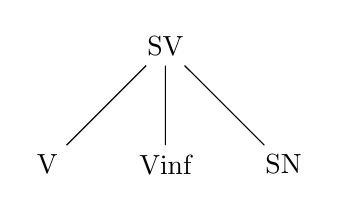
\begin{tikzpicture}
  \node{SV}
    child {node {V}}
    child {node {Vinf}}
    child {node {SN}}
  ;
\end{tikzpicture}
\caption{Exemple de structure plate.}
\end{figure}

Cette structure s'oppose à la structure hiérarchique suivante :\\

\begin{figure}[ht]
\centering
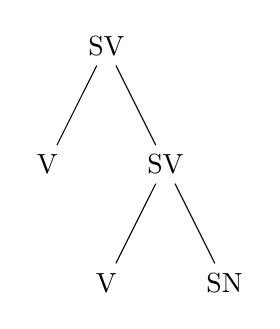
\begin{tikzpicture}
  \node{SV}
    child {node {V}}
    child {node {SV}
      child {node {V}}
      child {node {SN}}
    }
  ;
\end{tikzpicture}
\caption{Exemple de structure hiérarchique.}
\end{figure}


Une telle structure ne permet pas d'illustrer les phénomènes auxquels nous avons à faire car dans un tel cas, le verbe \emph{faire} ne pourrait pas récupérer les arguments du second verbe et en faire, notamment, ses clitiques.

Pour que les compléments du second verbe soient pronominalisés devant l'ensemble du groupe verbal, il faut que toutes les branches de l'arbre soient au même niveau.\\

Au niveau sémantique, enfin, on peut dire que le verbe \emph{faire} est une forme verbale qui exprime le fait que le sujet (par exemple \emph{Paul}) fait en sorte que d'autres fassent l'action à sa place.

Le sujet grammatical est appelé le 'causer' et le groupe nominal qui est le sujet initial du second verbe est appelé le 'causee'.
Dans l'exemple 1 (\autoref{phenomene.exemples}), c'est Paul qui est le 'causer' et c'est l'enfant qui est le 'causee'.



\subsection{Le phénomène linguistique : les difficultés empiriques}

Etant donné l'analyse linguistique que l'on vient de faire, on voit aisément que l'analyse HPSG va devoir faire face à quelques difficultés empiriques.
On peut en énumérer quelques unes :\\

\begin{itemize}
  \item les clitiques ne doivent pas être rattachés au verbe dont ils sont les compléments mais au verbe \emph{faire}.
    Cela nécessiste, comme on vient de le voir, la mise en place d'une structure plate
  \item il faudra également distinguer les constructions dans lesquelles interviennent des verbes instransitifs des constructions dans lesquelles interviennent des verbes transitifs directs
  \item le sujet du second verbe n'est pas à sa place canonique mais est placé après le verbe et ses compléments, si il y en a.\\
    En plus de boulverser l'ordre canonique des compléments, cette modification fait aussi varier la forme des pronoms clitiques.
\end{itemize}


\subsection{Les motivations théoriques de l'analyse HPSG, les grands principes de l'analyse et le dispositif formel}

HPSG propose une solution pour représenter les phénomènes présents dans une structure causative et rejeter les phrases jugées non grammaticales qui semble particulièrement bien adaptée.\\

HPSG permet notamment de faire de la composition argumentale et sait décrire les performances linguistiques.
En effet, les descriptions sont déclaratives, ont un ordre indépendant et sont réversibles.
HPSG utilise des structures de traits pour définir à la fois les mots et les phrases.

Alors que la grammaire générative a des problèmes depuis plus de 25 ans avec les affixes pronominaux, HPSG propose là aussi des solutions.
En effet, HPSG propose une structure syntaxique qui fournit les outils nécessaires pour gérer la distribution des affixes pronominaux sans violer leur intégrité lexicale.
HPSG utilise une analyse purement lexicaliste et ne fait appel à aucune règle de mouvement.\\

HPSG  analyse les verbes comme têtes de phrase.
Dans le cas particulier des constructions causatives, on considère que le verbe, ici \emph{faire}, sélectionne un verbe à l'infinitif ainsi que les compléments de ce verbe.
De plus, en tant que tête, \emph{faire} contrôle l'accord avec le sujet et transmet à la phrase son mode.
On considère que le verbe à l'infinitif transfère sa sous catégorisation au verbe \emph{faire}.

On a donc la structure suivante :

\begin{figure}[ht]
\centering
\begin{minipage}{.8\textwidth}
\centering
\begin{avm}
			sous-cat  < V [{v}
                                       MODE & inf\\
                                       sous-cat & L
                                      ] > + L
\end{avm}
\caption{Sous-catégorisation de \emph{faire} comprenant un verbe à l'infinitif et la sous-catégorisation de ce verbe ('L' représente la liste des arguments du verbe à l'infinitif)}
\end{minipage}
\end{figure}


Le verbe \emph{faire} sélectionne le verbe à l'infinitif et remonte dans sa liste de sous catégorisation tous les arguments du verbe à l'infinitif.
Par exemple, si le verbe à l'infinitif a dans sa sous catégorisation : <SN, SN>, \emph{faire} aura dans la sienne : <V, SN, SN>.

Après l'aspiration des compléments, la séquence \emph{faire} + verbe à l'infinitif se comporte comme un verbe transitif.
La liste de sous catégorisation du verbe à l'infinitif pourra rester non saturée car la branche de cet élément n'est pas une branche tête.\\

On dit généralement que les langages se distinguent dans leur manière de représenter les arguments.

HPSG a l'avantage de distinguer à la fois la sous catégorisation et la valence d'un verbe.
La présence d'un trait représentant la valence et d'un autre trait représentant la sous catégorisation permet d'enregistrer des décalages entre les arguments attendus et ceux qui sont réalisés.
En formulant des contraintes, HPSG autorise donc, notamment quand il y a des affixes, des manipulations à ce niveau.\\

On distingue donc les mots simples notés \emph{pl-wd} et les mots cliticisés \emph{cl-wd}.
Les mots cliticisés sont des verbes.
Il existe une notation pour les clitiques sujets et une pour les clitiques objets, respectivement : \emph{su-cl-wd} et \emph{non-su-cl-wd}.\\

Les clitiques sont considérés comme des éléments non canoniques et plus précisément comme des affixes pronominaux faisant partie de la flexion du verbe.
Leur synsem est particulier : \emph{aff-synsem} (pour affixal synsem).

Si un verbe porte un clitique, il change de type en devenant un v-cliticisé.
Ce type permet à HPSG d'imposer des contraintes très utiles.

Les mots de type v-cliticisé doivent avoir un complément soustrait de leur liste COMPS.
Par conséquent, le complément n'apparaît que dans la liste SOUS-CAT du verbe qui porte le clitique.
Cela permet de dire que le verbe n'attend plus ce complément puisqu'il le porte déjà sur lui.
On peut montrer avec les portions de structures ci-dessous la différence qu'il existe entre un verbe transitif (\autoref{phenomene.nclit}) et le même verbe cliticisé (\autoref{phenomene.clit}) :\\

\begin{figure}[ht]
\centering
\begin{avm}
  [{}
    Phon & </\emph{mange}/> \\
    Synsem = Cat & [{cat}
                    sous-cat & < SN {1}, SN {2} >
                   ]
  ]
\end{avm}
\caption{Verbe non cliticisé, attendant deux compléments\label{phenomene.nclit}}
\end{figure}
\begin{figure}[ht]
\centering
\begin{avm}
  [{}
    Phon & </\emph{le mange}/> \\
    Synsem & [{synsem}
              Local = Cat & [{cat}
                             sous-cat < SN {1} >
                            ] \\
              Non local & [{nloc}
                           CL < SN {2} >
                          ]
             ]
  ]
\end{avm}
\caption{Verbe cliticisé (portant un clitique, soustrait de la liste des compléments)\label{phenomene.clit}}
\end{figure}

On notera que HPSG permet aux phénomènes de valence d'être traités dans le lexique.
La valence désigne tous les éléments avec lesquels le signe doit se combiner pour être complet.\\

Les arguments qui sont extraits ne sont pas représentés par des branches vides, c'est un des principes de HPSG : il ne doit pas y avoir de branche vide.
A la place, les arguments extraits sont enregistrés dans l'entrée lexicale.

Ces informations sont plus précisément enregistrées dans le trait NON-LOCAL (SLASH).
Le trait NON-LOCAL enregistre la valeur de l'argument extrait.
Ainsi, grâce au principe de trais de tête, les informations portées par le verbe à ce sujet vont remonter et être partagées par toutes les têtes, jusqu'au sommet de la dépendance.
Ce mécanisme est particulièrement utile dans les phrases qui contiennent des enchassements car on ne perd pas d'informations en faisant remonter les informations par les têtes.\\

Enfin, on remarquera que HPSG a une architecture double (inventaire raisonné des différentes unités constititives et principe de combinaison des unités entre elles) qui permet de ne traiter que les objets bien formés.
On ne trouvera pas de description possible pour un objet mal formé : soit l'objet n'existe pas, soit aucune combinaison ne l'autorise.
